\documentclass[titlepage,a4paper]{article}

\usepackage{a4wide}
\usepackage[colorlinks=true,linkcolor=black,urlcolor=blue,bookmarksopen=true]{hyperref}
\usepackage{bookmark}
\usepackage{fancyhdr}
\usepackage[spanish]{babel}
\usepackage[utf8]{inputenc}
\usepackage[T1]{fontenc}
\usepackage{graphicx}
\usepackage{float}

\pagestyle{fancy} % Encabezado y pie de página
\fancyhf{}
\fancyhead[L]{TP2 - Grupo 11}
\fancyhead[R]{Algoritmos y Programación III - FIUBA}
\renewcommand{\headrulewidth}{0.4pt}
\fancyfoot[C]{\thepage}
\renewcommand{\footrulewidth}{0.4pt}

\begin{document}
\begin{titlepage} % Carátula
	\hfill
\includegraphics[width=6cm]{logofiuba.jpg}
    \centering
    \vfill
    \Huge \textbf{Trabajo Práctico 2 — Java}
    \vskip2cm
    \Large [7507/9502] Algoritmos y Programación III\\
    Curso 2 \\ % Curso 1 para el de la tarde y 2 para el de la noche
    Segudo cuatrimestre de 2019 
    \vfill
    \begin{tabular}{ | l | l | l | } % Datos del alumno
      \hline \hline
      Alumno & Número de padrón & Email\\ \hline \hline
      CLAROS, ELVIS&99879&eclaros@fi.uba.ar\\ \hline
      BARRIO, HERNÁN&89317&hbarrio86@gmail.com\\ \hline
      MENDEZ, GABRIELA&101741&gabrielamendezg@outlook.com\\ \hline
      MARTINEZ, SELENE&100439&zeluuh@gmail.com\\ \hline
  	\end{tabular}
    \vfill
    \vfill
\end{titlepage}

\tableofcontents % Índice general
\newpage

\section{Introducción}\label{sec:intro}
El presente informe reúne la documentación de la solución del segundo trabajo práctico de la materia Algoritmos y Programación III que consiste en desarrollar una aplicación de un Juego de Tablero con nombre \textbf{AlgoChess} en Java utilizando los conceptos del paradigma de la orientación a objetos vistos en el curso.

\section{Supuestos}\label{sec:supuestos}
% Deberá contener explicaciones de cada uno de los supuestos que el alumno haya tenido que adoptar a partir de situaciones que no estén contempladas en la especificación.

\begin{itemize}
\item Solo existe una instancia del juego al mismo tiempo en el programa.
\item Solo existen y deben existir 2 jugadores durante el transcurso del juego.
\item Cada Jugador intercambia todos sus puntos y coloca las piezas adquiridas únicamente en la fase inicial del juego.
\item No existen restricciones en la elección y cantidad de cada unidad más allá de los puntos que posee el jugador para "comprarlas".
\item En su turno el jugador solo puede realizar movimientos con una unidad (o batallón).
\item En su turno el jugador puede realizar alguna de las siguientes acciones, una vez realizada no tiene más acciones disponibles: 
\begin{itemize}
\item Solo mover una unidad.
\item Solo atacar.
\item Mover y luego atacar con la misma unidad.
\end{itemize}
\item El jugador (actor externo al programa) indica cuando termina su turno.
\item Batallón solo pude formarse con 3 soldados de infantería contiguos en horizontal.
\item Batallón solo puede moverse en conjunto, pero solo se puede atacar con el soldado especifico seleccionado. 
\end{itemize}

\section{Diagramas de clase}\label{sec:diagramasdeclase}
% Uno o varios diagramas de clases mostrando las relaciones estáticas entre las clases.  Puede agregarse todo el texto necesario para aclarar y explicar su diseño. Recuerden que la idea de todo el documento es que quede documentado y entendible cómo está implementada la solución.
A continuación se exhiben algunos diagramas de clases:


\begin{figure}[H]
\centering
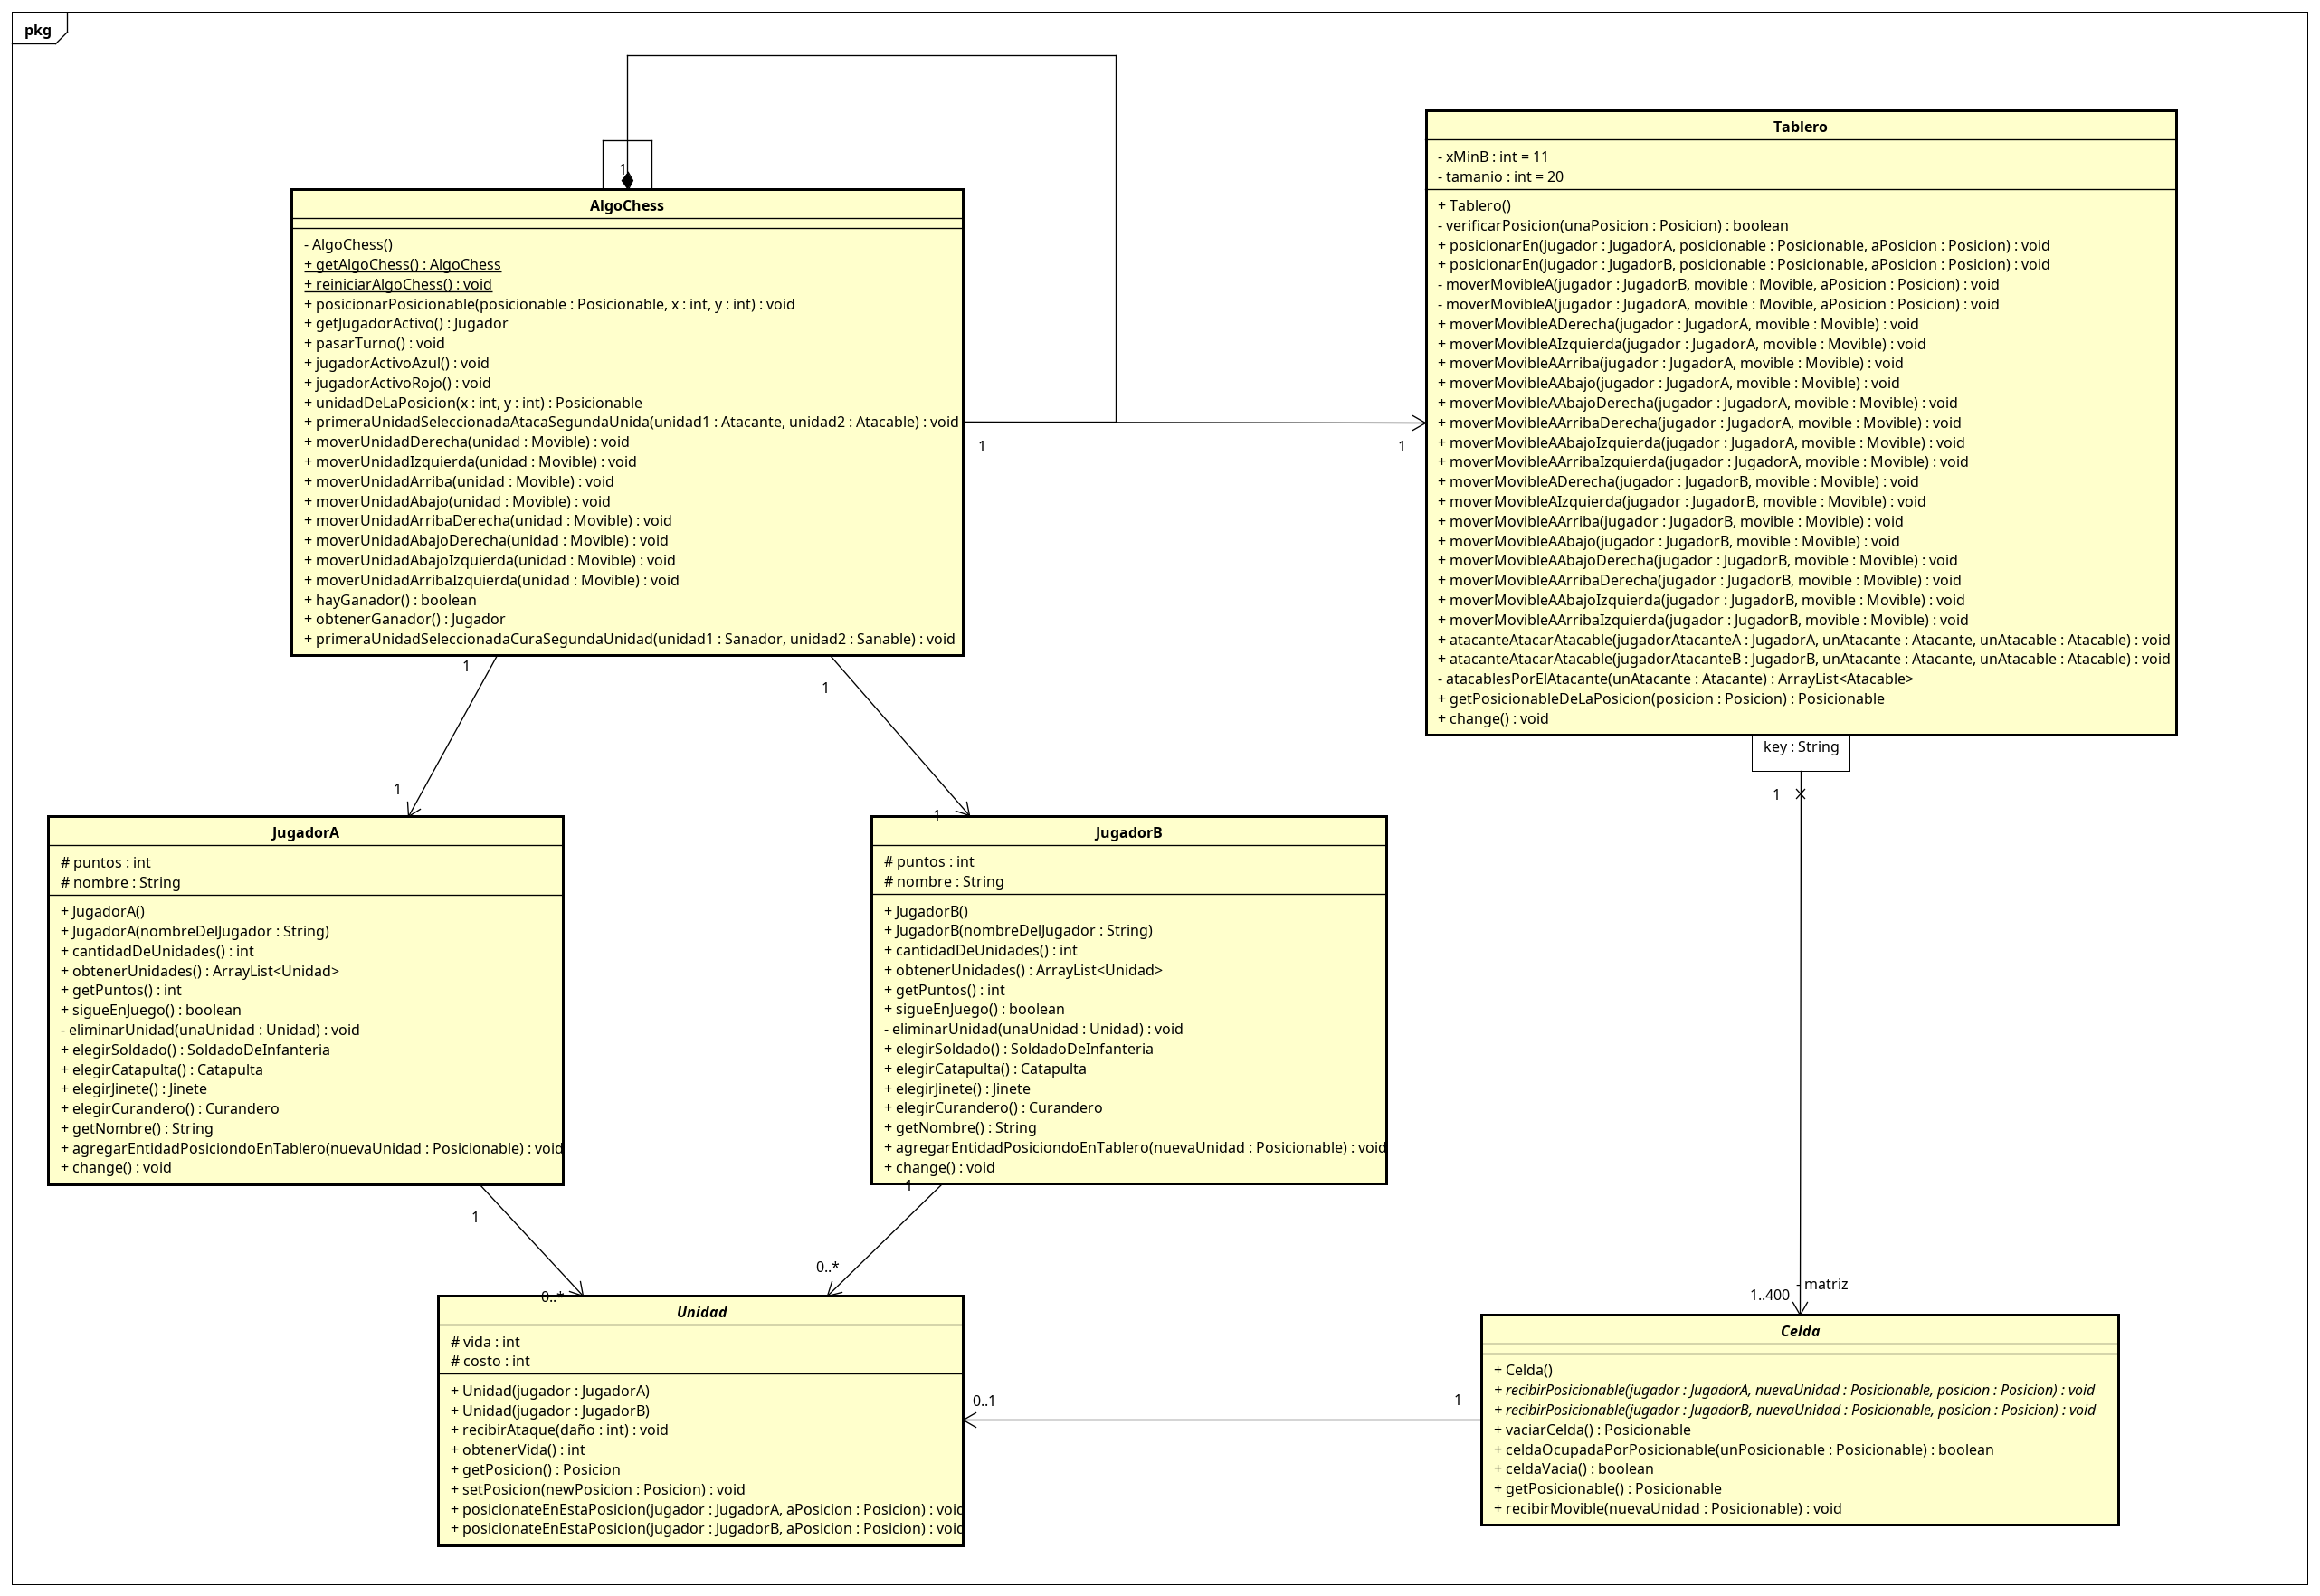
\includegraphics[width=0.8\textwidth]{DiagramasDeSecuencia/DiagramaDeClasesPrincipalModelo.png}
\caption{\label{fig:class01q}Diagrama de Clases del modelo principal.}
\end{figure}
 
\begin{figure}[H]
\centering
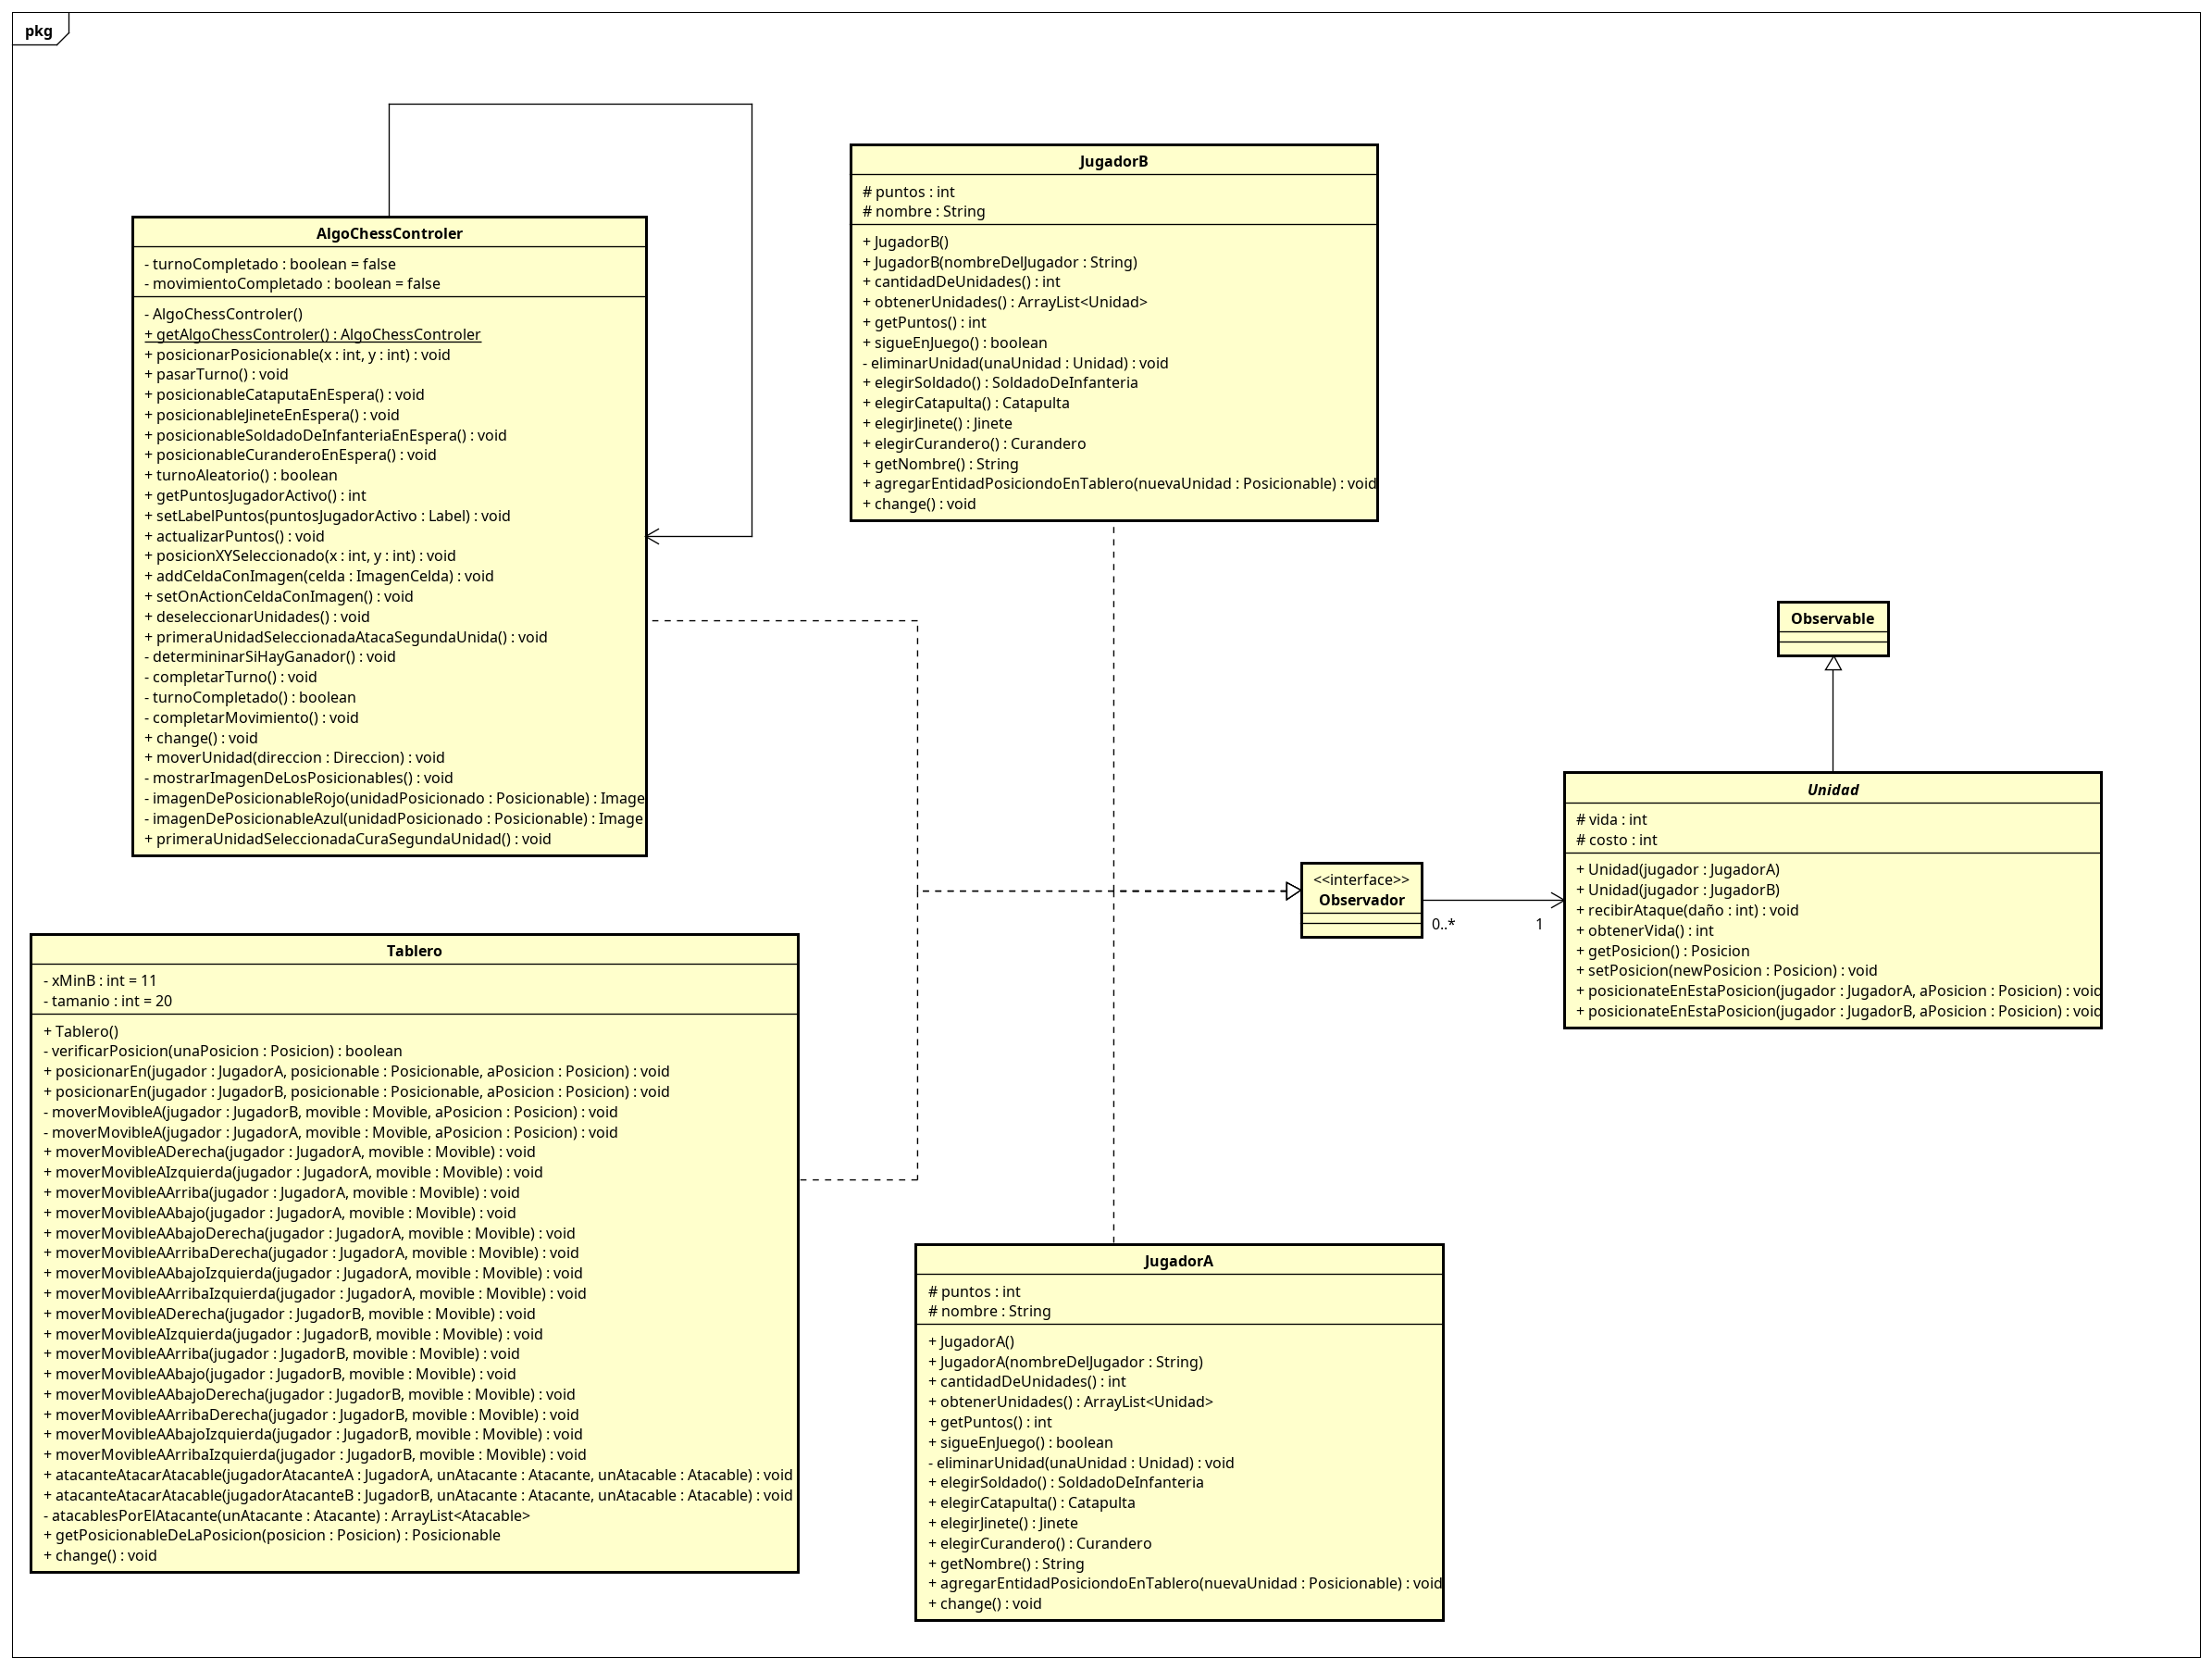
\includegraphics[width=0.8\textwidth]{DiagramasDeSecuencia/ObserverObservador.png}
\caption{\label{fig:class01p}Relación observador y observado.}
\end{figure}

\begin{figure}[H]
\centering
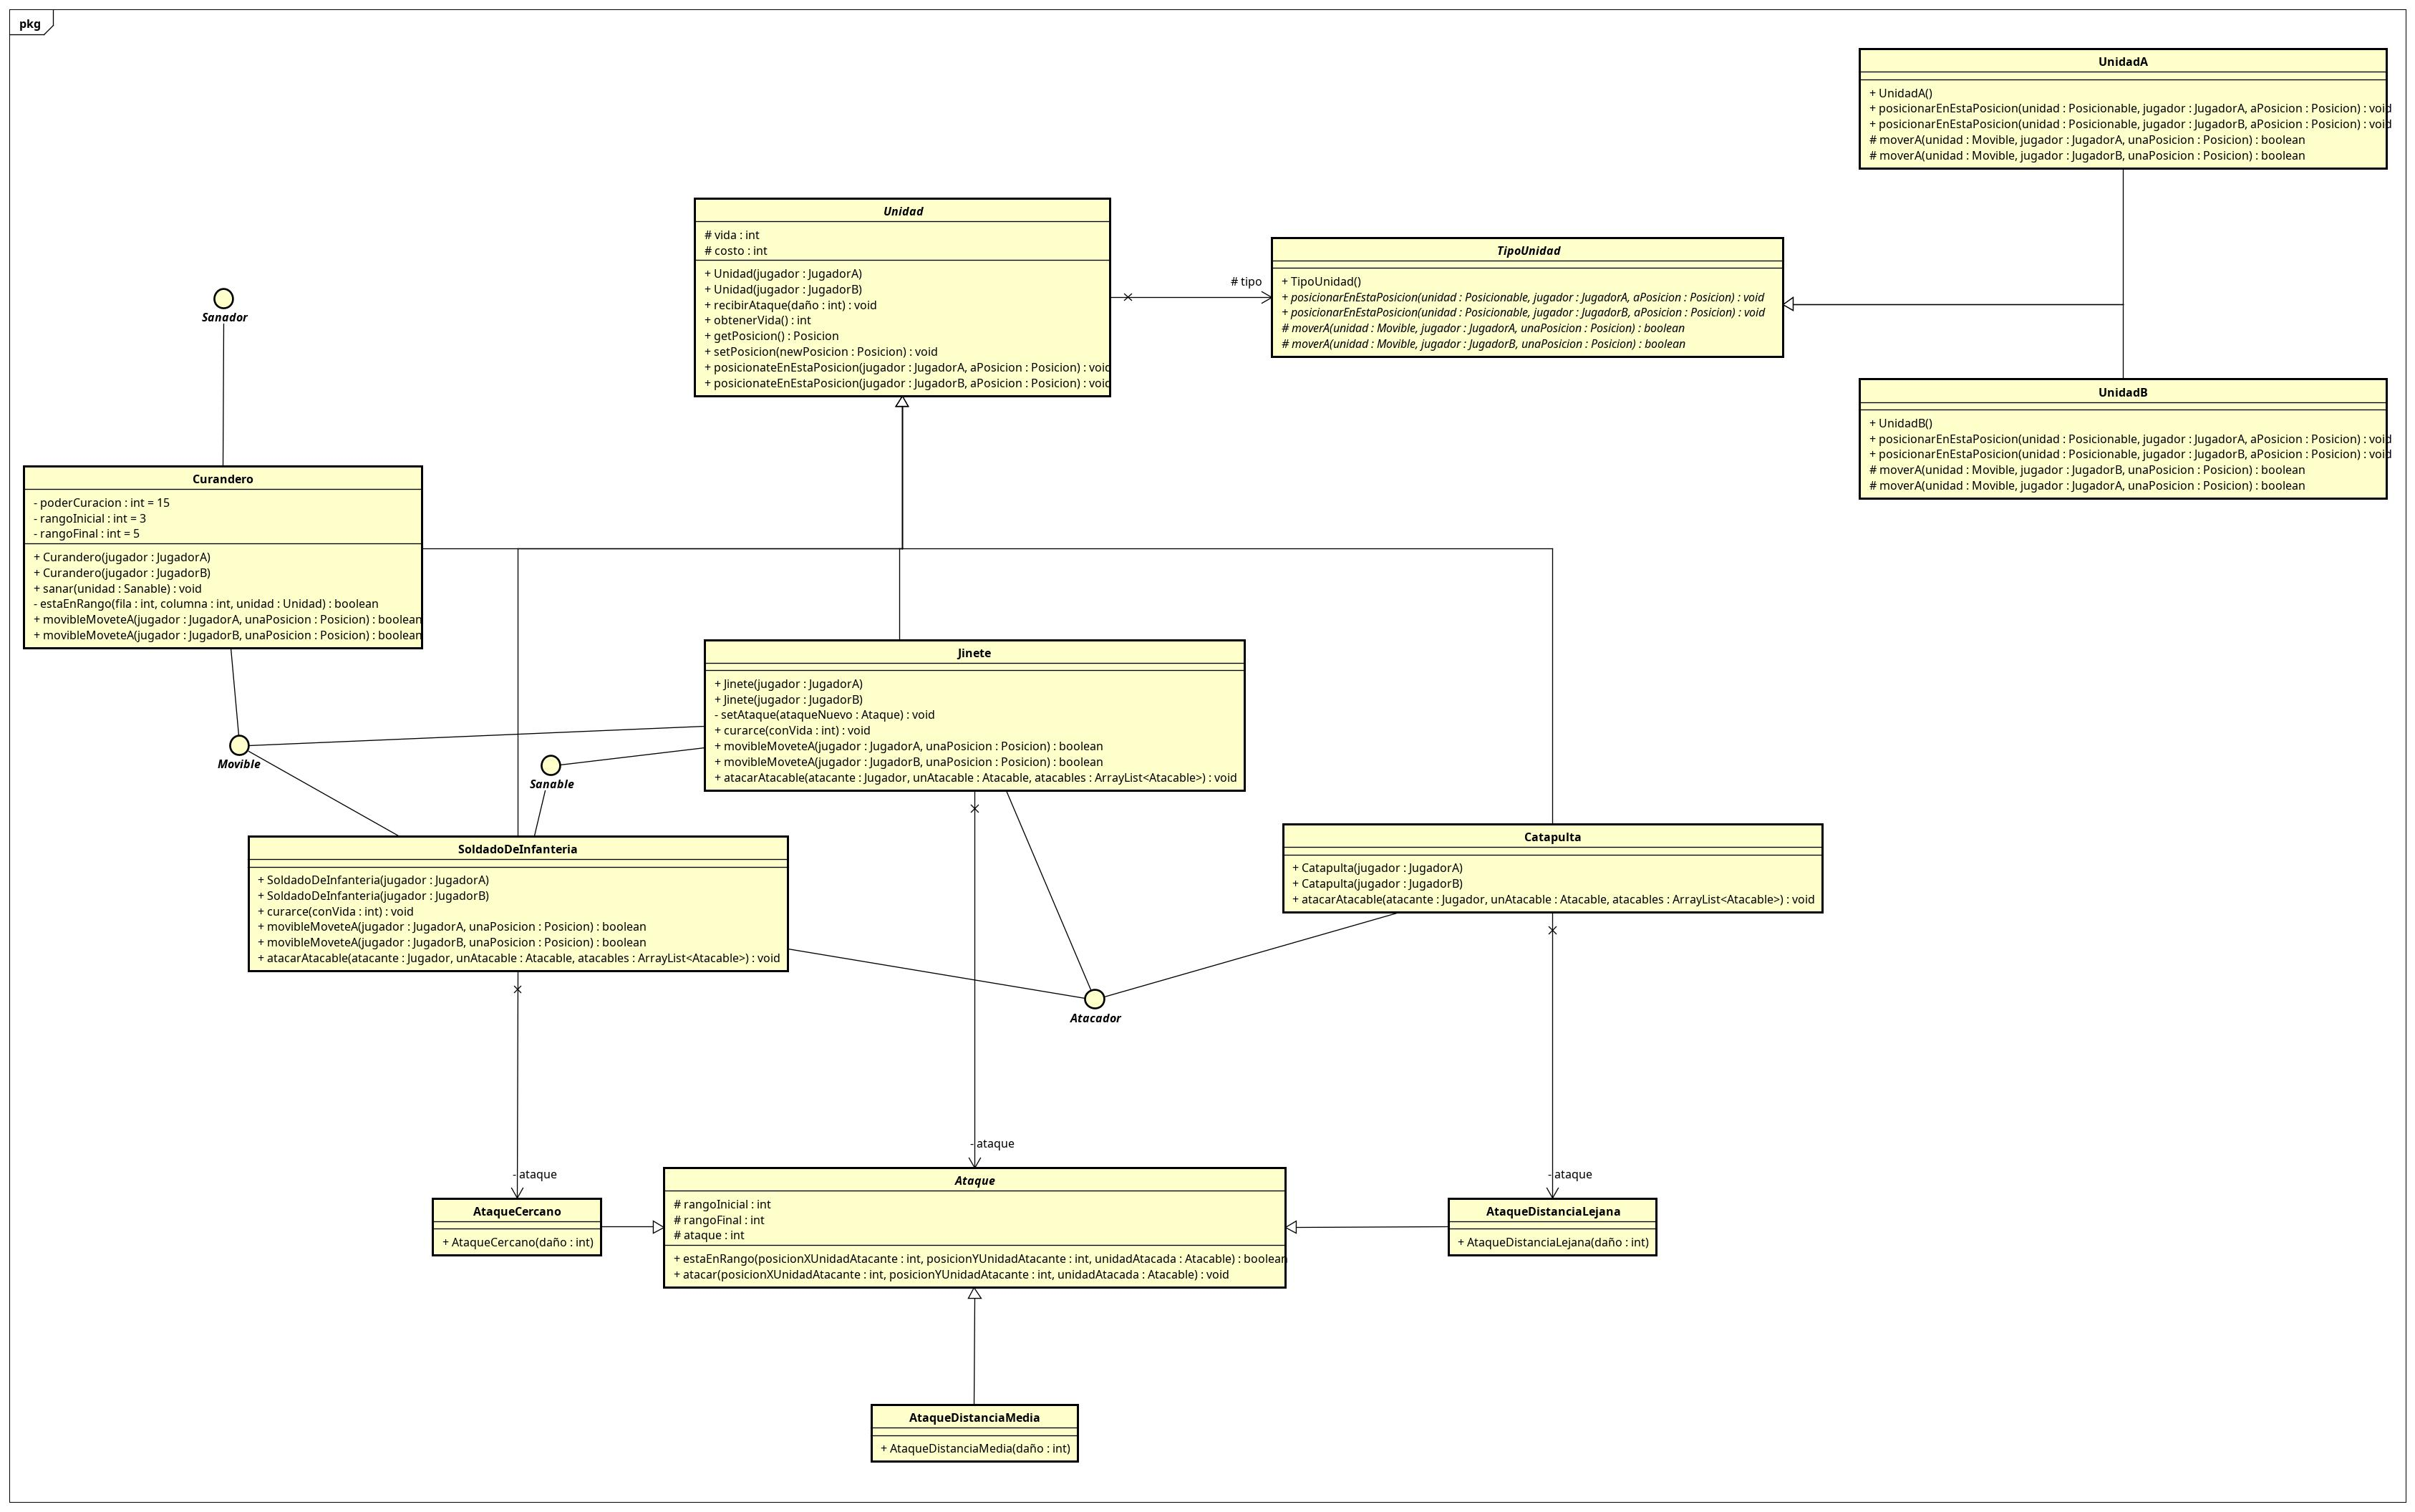
\includegraphics[width=0.8\textwidth]{DiagramasDeClases/28-nov clases entidades y ataque.jpg}
\caption{\label{fig:class01o}Diagrama de Unidades y Ataque.}
\end{figure}

\begin{figure}[H]
\centering
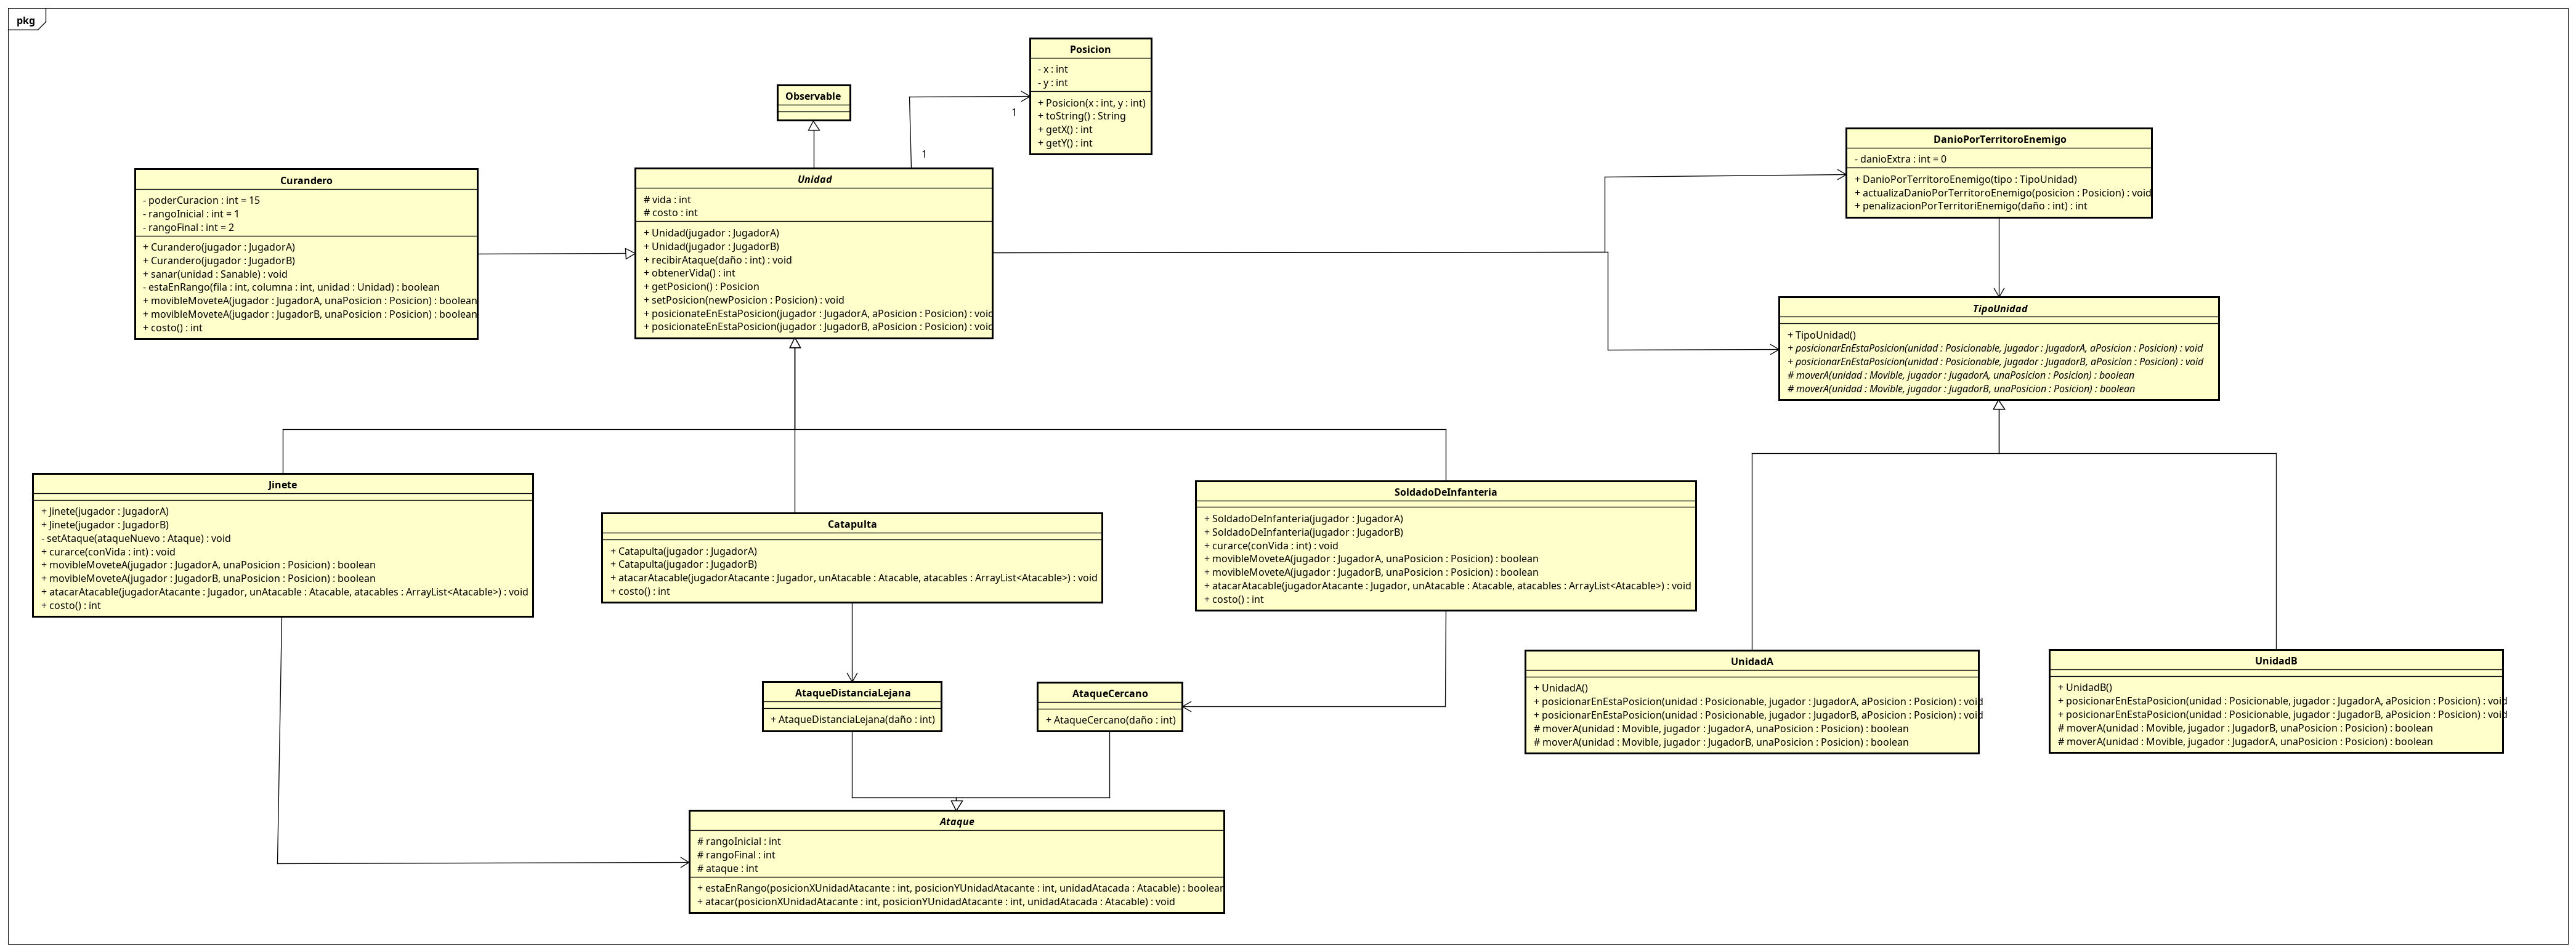
\includegraphics[width=0.8\textwidth]{DiagramasDeSecuencia/EntidadesAtaquesTipos.png}
\caption{\label{fig:class01i}Diagrama de Unidades, Ataque y su correspondiente relación con los tipos .}
\end{figure}

\begin{figure}[H]
\centering
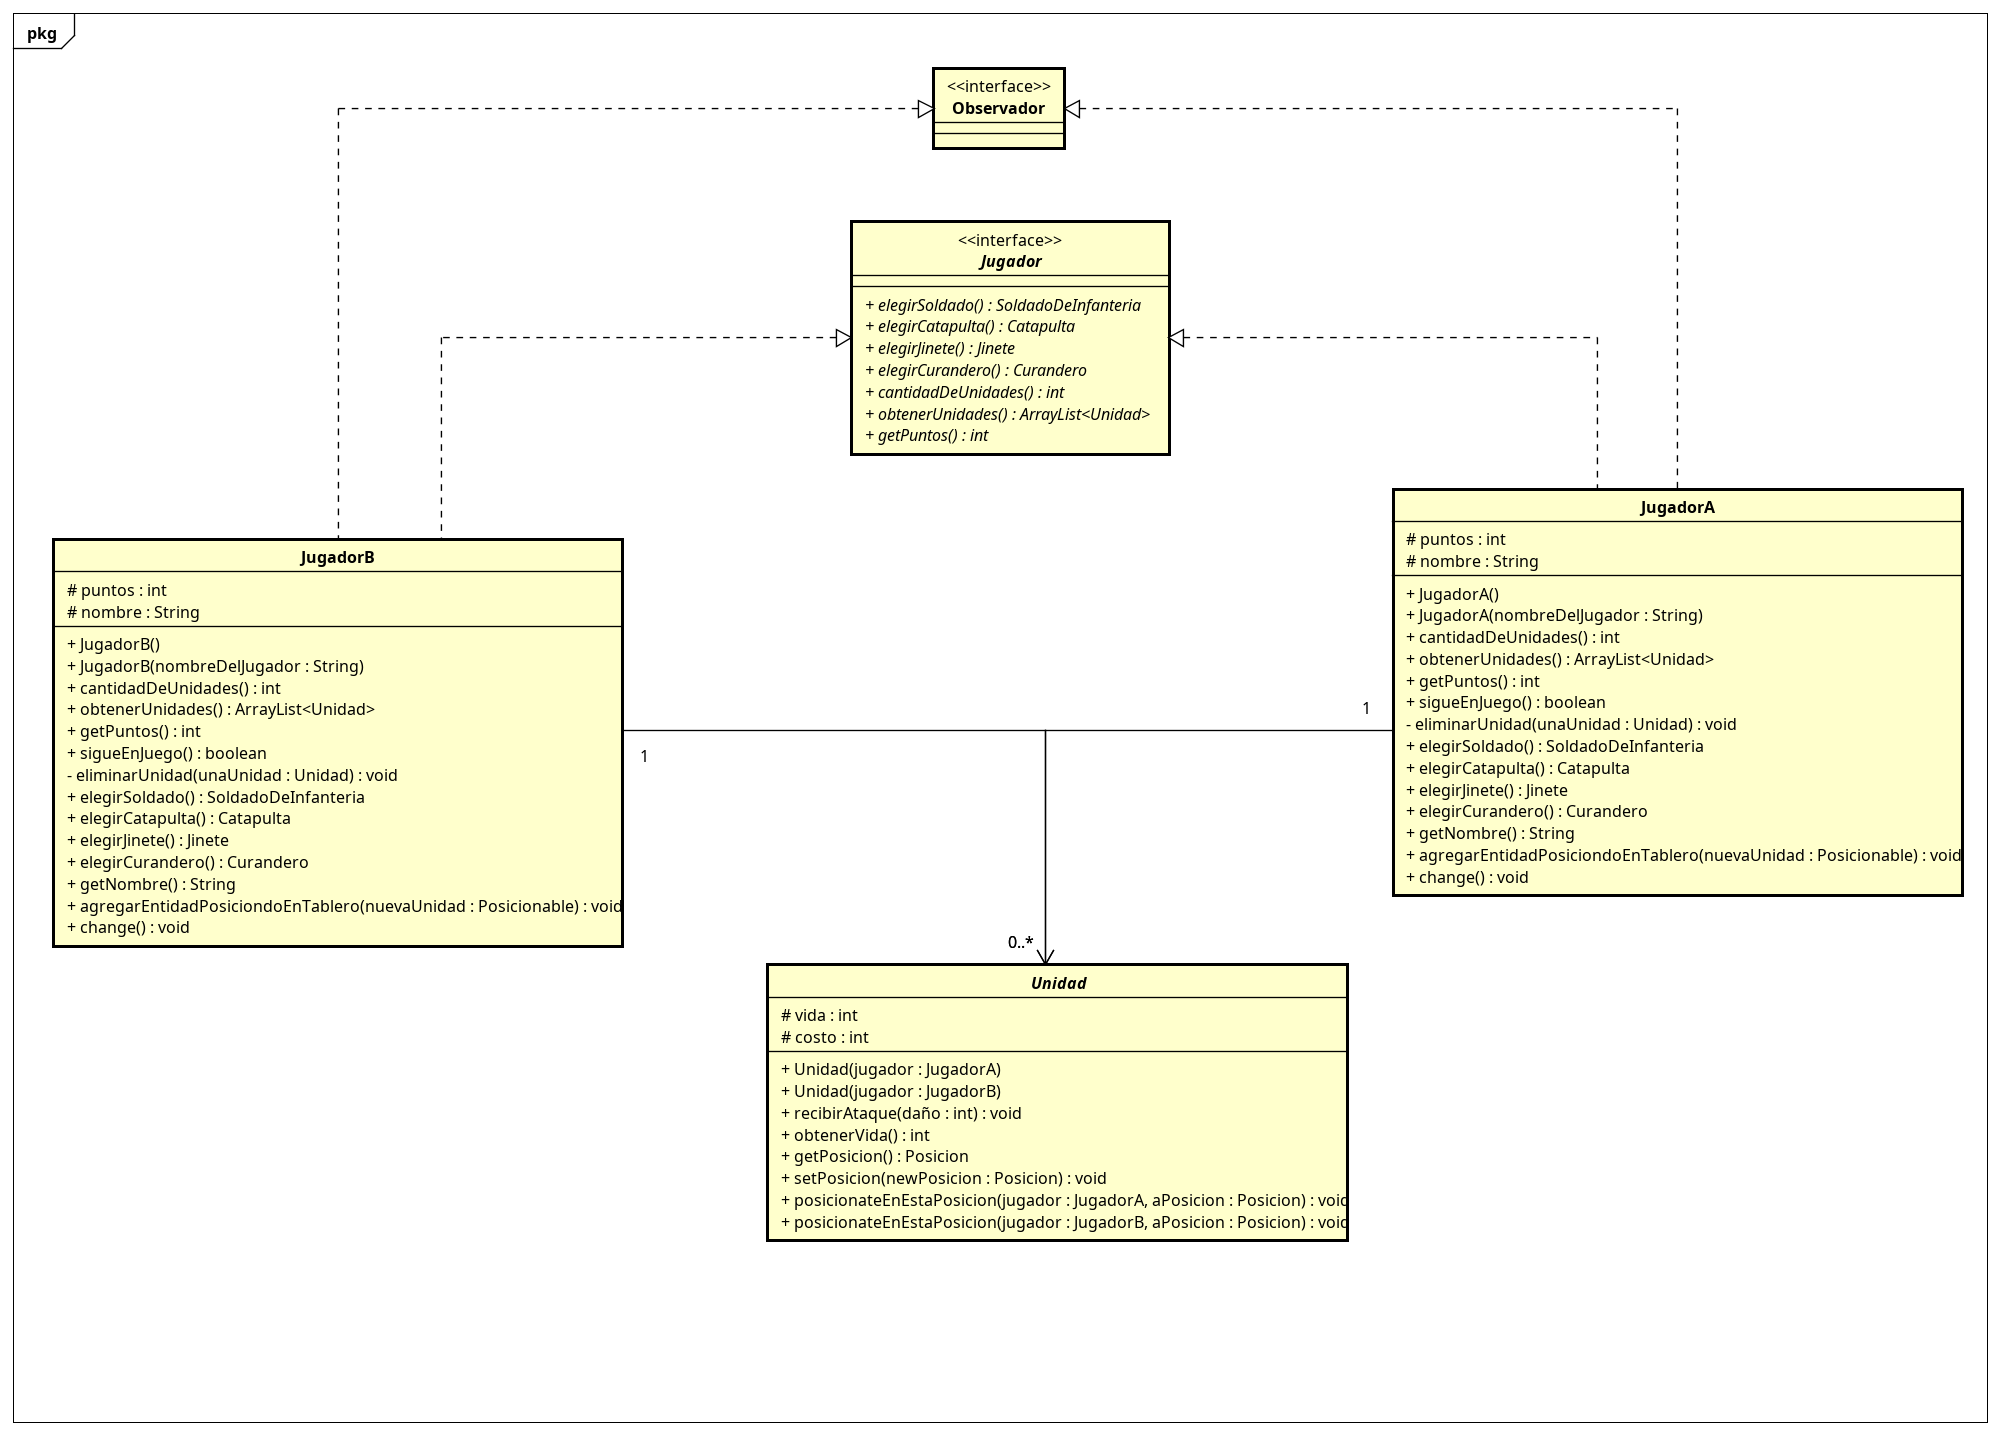
\includegraphics[width=0.8\textwidth]{DiagramasDeSecuencia/JugadoresUnidad.png}
\caption{\label{fig:class01u}Diagrama de Unidades y Jugador la relación que tienen .}
\end{figure}


\section{Diagramas de secuencia}\label{sec:diagramasdesecuencia}
% Mostrar las secuencias interesantes que hayan implementado. Pueden agregar texto para explicar si algo no queda claro.
Los siguientes diagramas ilustran secuencias de la primera entrega de TP2

\begin{figure}[H]
\centering
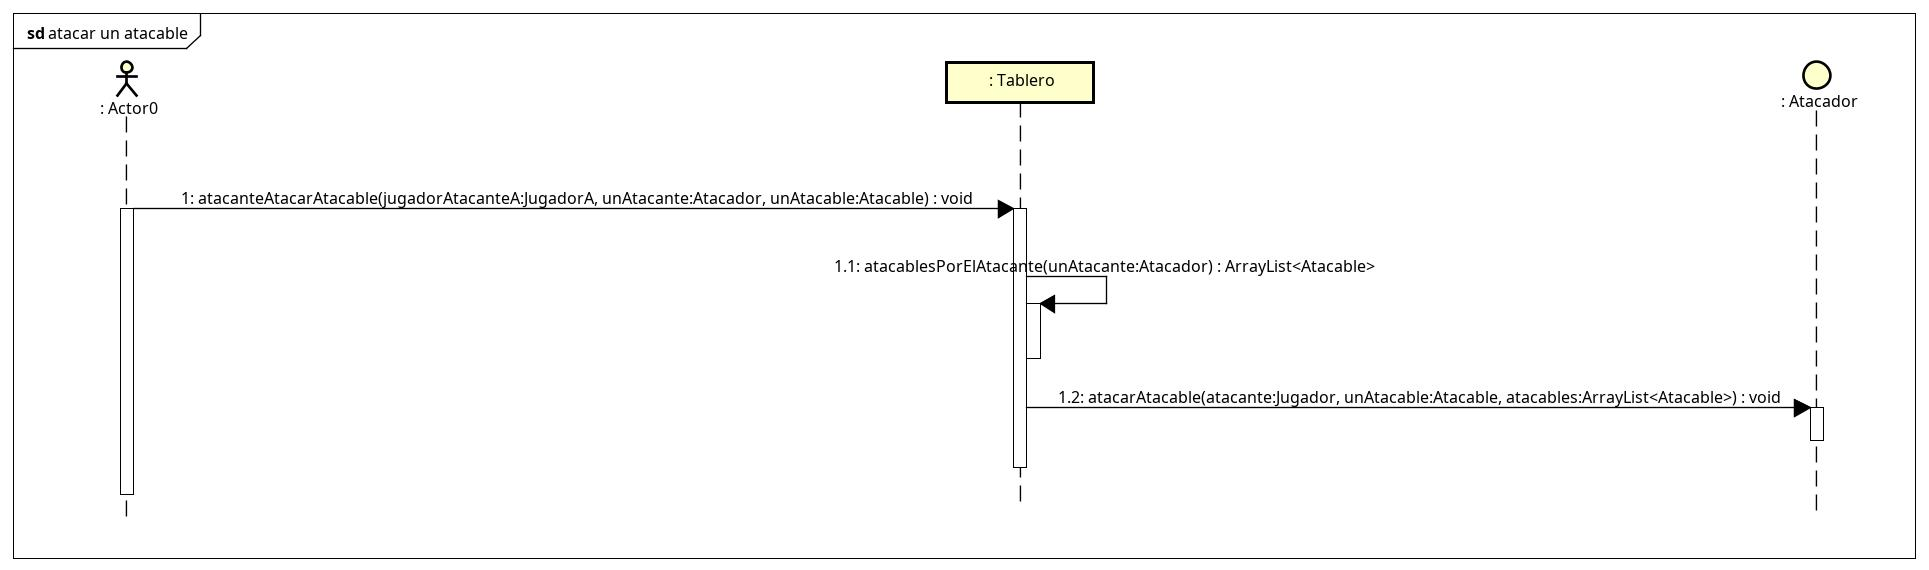
\includegraphics[width=0.8\textwidth]{DiagramasDeSecuencia/28-nov atacar un atacable.jpg}
\caption{\label{fig:seq01y}Secuencia de ataque a una entidad atacable.}
\end{figure}

En el diagrama  \ref{fig:seq01t} se puede observar el ataque de una una unidad que implementa la interfaz "Atacador" a otra que implementa la interfaz "Atacable"


\begin{figure}[H]
\centering
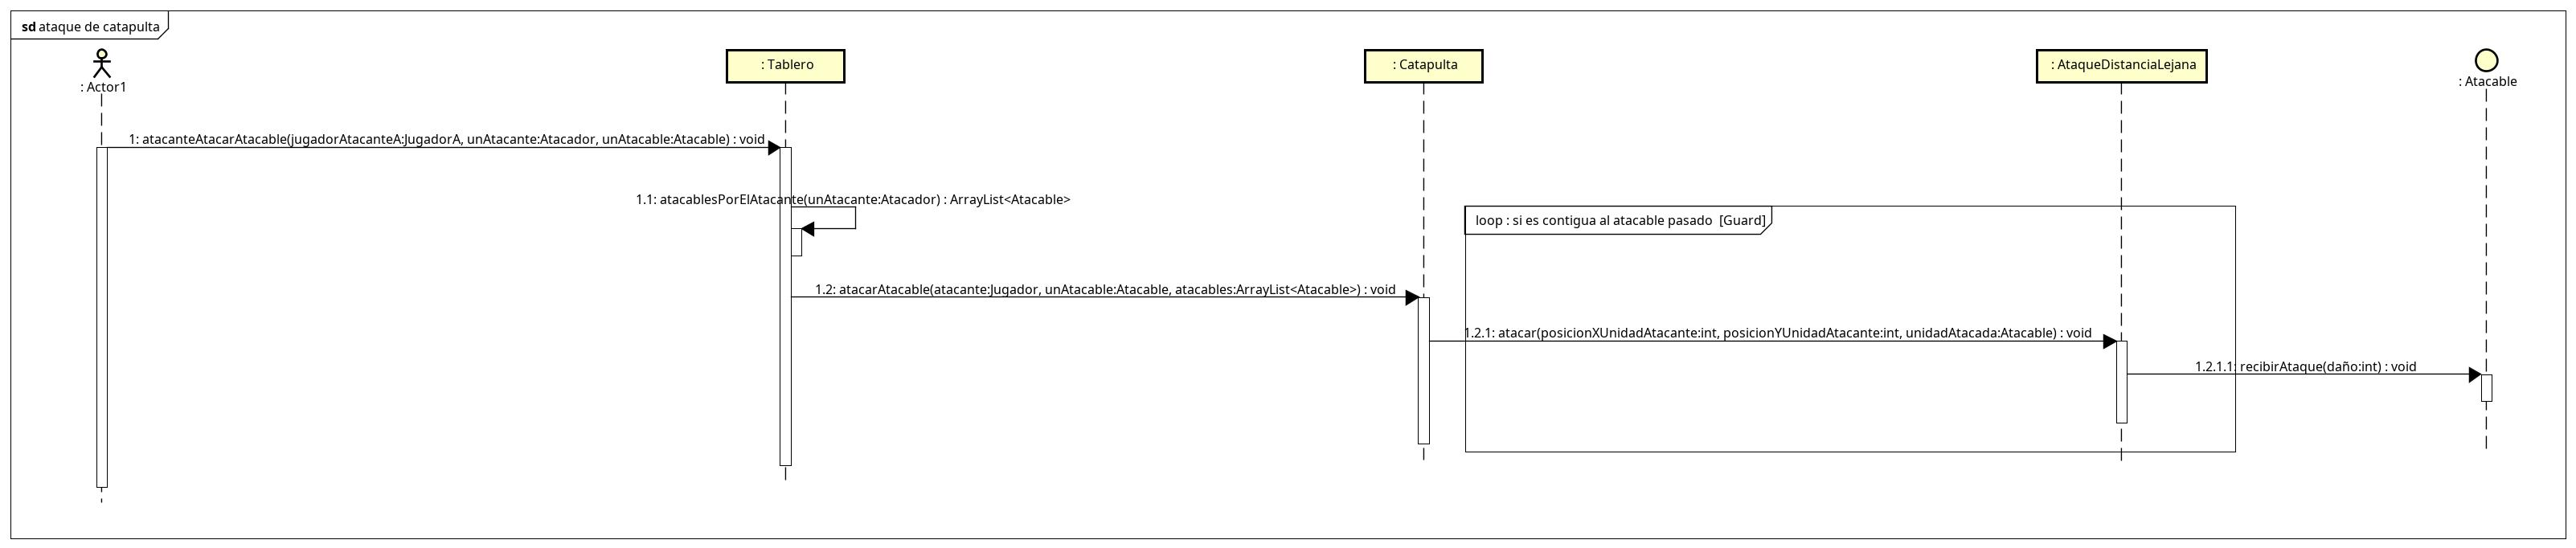
\includegraphics[width=\textwidth]{DiagramasDeSecuencia/28-nov ataque de catapulta.jpg}
\caption{\label{fig:seq02r}Secuencia de ataque de una catapulta.}
\end{figure}

En el diagrama  \ref{fig:seq02e} se puede observar el ataque catapulta a otra unidad "atacable".

\section{Diagrama de Paquetes}\label{sec:diagramadepaquetes}
% Incluir un diagrama de paquetes UML para mostrar el acoplamiento de su trabajo

En esta sección se presenta un diagrama general de la relación que excite entre los paquetes.

\begin{figure}[H]
\centering
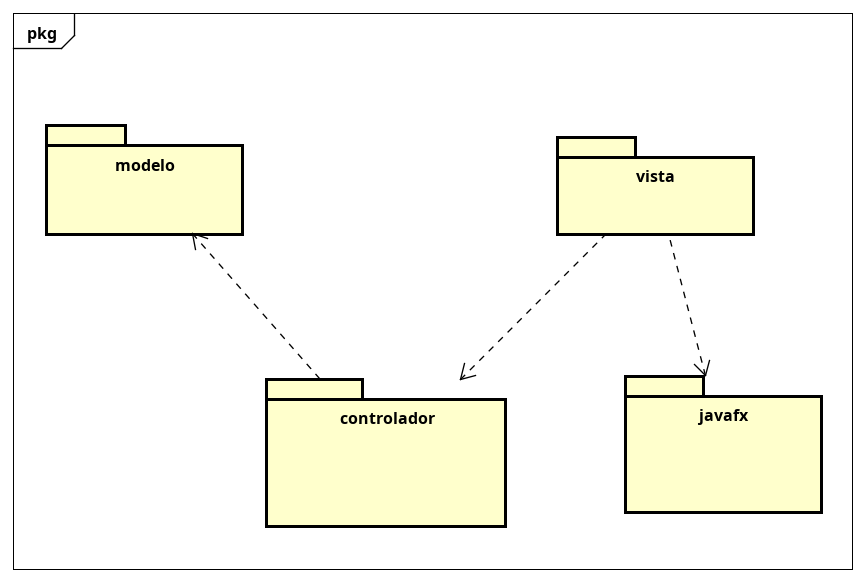
\includegraphics[width=\textwidth]{DiagramasDeSecuencia/Paquetes.png}
\caption{\label{fig:seq02w}Relación de los paquetes.}
\end{figure}

\section{Diagramas de Estado}\label{sec:diagramasdeestado}
% Incluir diagramas de estados, mostrando tanto los estados como las distintas transiciones para varias entidades del modelo.

Se tiene los estados que la Celda puede tomar en el siguiente diagrama.

\begin{figure}[H]
\centering
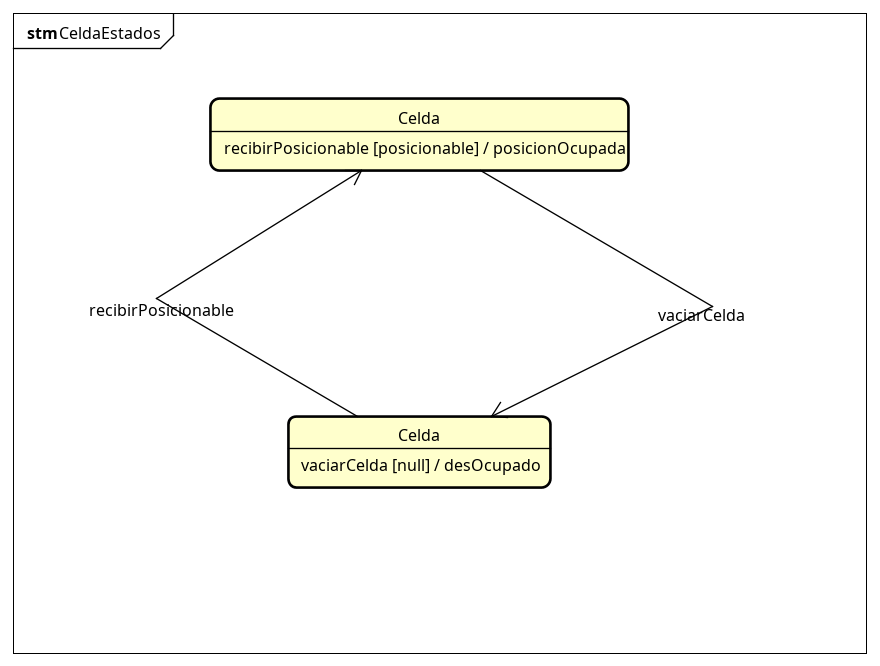
\includegraphics[width=\textwidth]{DiagramasDeSecuencia/CeldaEstadosV2.png}
\caption{\label{fig:seq02q}Estados de la Celda.}
\end{figure}

\section{Detalles de implementación}\label{sec:implementacion}
% Explicaciones sobre la implementación interna de algunas clases que consideren que puedan llegar a resultar interesantes.

\subsection{Tablero}
Esta clase Tablero implementa las posiciones del mismo a partir de un HashMap <String, Celda> matriz. Inicializa el tablero donde se desarrollara el juego, manipula "Posicion(es)" al realizar el posicionamiento de las Unidades al comienzo de la partida y durante la misma (con Unidades que implementan las interfaces "Posicionable" y "Movible". Los metodos publicos que permiten realizar movimientos son los que mueven unidades en cada direccion vertical, horizontal y diagonales (ejemplo adelante). Por ultimo, la clase Tablero se ocupa del comportamiento del Batallon junto con la clase MovimientoDeBatallonDeSoldadosDeInfanteria.

\begin{verbatim}
public void moverMovibleAArribaDerecha(JugadorB jugador, Movible movible) {
		moverMovibleA(jugador, movible, new Posicion(movible.getPosicion().getX() + 1, movible.getPosicion().getY() + 1));
	}
\end{verbatim}

\subsection{Jugador}
Jugador es una una interfaz que es implementada por las clases JugadorA y JugadorB, que encapsulan el comportamiento de los dos jugadores que existiran durante la partida. Tienen la responsabilidad de gestionar la eleccion de sus unidades durante la seleccion al comienzo de la partida, ademas de guardar a las mismas.

\subsection{Unidad}
 Para las unidades implementamos una clase abstracta Unidad de la cual heredan los métodos sus clases hijas.
  \begin{enumerate}
      \item SoldadoDeInfanteria
      \item Jinete
      \item Catapulta
      \item Curandero
  \end{enumerate}
Todas las unidades implementan la interfaz "Posicionable" y tienen la responsabilidad de gestionar su vida como su posicionamiento (durante la fase de posicionar unidades). Las clases hijas implementan distintas interfaces que determinan su comportamiento (Atacable, Atacador, Movible, Sanable, Sanador). A su vez cada unidad consta de un TipoDeUnidad que indica a que jugador pertenece.
\subsection{Unos detalles mas}
Para la distancia de los ataques se implementaron tres clases (AtaqueCercano, AtaqueDistanciaLejana, AtaqueDistanciaMedia) que heredan de Ataque, y encapsulan el rango de los ataques correspondientes a las distintas Unidades del juego.



\section{Excepciones}\label{sec:excepciones}
% Explicación de cada una de las excepciones creadas y con qué fin fueron creadas.

\begin{description}
\item[CoordenadaFueraDelTableroException] 
\item[FilaOColumnaNoPerteneceATuParteDelTableroExcepcion]
\item[FueraDelRangoDeAtaqueExcepcion] 
\item[InstanciaDeTableroYaExiste] 
\item[NoEsTuUnidadExcepcion] 
\item[NoMePuedesMoverNoEresMiDuenioExcepcion] 
\item[PosicionOcupadaExcepcion] 
\item[PuntosInsuficientesExcepcion] 
\item[SoloTePuedesMoverUnaPosicionExcepcion] 





\end{description}

\end{document}
